\section{Ablation: Published Losses on a Fixed 3M Encoder}
\label{sec:ablation}

We compare representative \textbf{published SSL objectives} under identical
conditions: SmallResNet ($\sim$2.8M params), CIFAR-100, block masking,
predictor-corrupt alignment where applicable, and the evaluation protocol of
Section~\ref{sec:evaluation}.
The primary comparison point is \textbf{200 training epochs}; preliminary
100-epoch numbers from completed runs are included where 200-epoch checkpoints
are still pending.

\subsection{Methods compared}
\label{sec:ablation-methods}

Table~\ref{tab:ablation-methods} lists each row, the loss family, and the
config file used to reproduce the run.
All single-encoder rows share \texttt{anchor\_mode=predictor\_corrupt} except
VICReg-encoder and JEPA-encoder ablations.

\begin{table*}[t]
  \centering
  \caption{Ablation methods on the shared 3M SmallResNet.
  ``Views'' indicates which inputs are encoded each step.
  EMA-JEPA uses a separate teacher encoder (not counted in trainable params).}
  \label{tab:ablation-methods}
  \small
  \begin{tabular}{llllp{5.8cm}}
    \toprule
    Method & Family & Views & Config & Loss (summary) \\
    \midrule
    JEPA cosine & Predictive~\cite{assran2023ijepa}
      & $x_c, \tilde{x}$
      & \texttt{single\_encoder\_jepa.json}
      & $\|g_\phi(z_c) - \sg(z)\|^2_{\cos}$ \\
    EMA JEPA & Predictive + teacher
      & $x_c, \tilde{x}$
      & \texttt{cifar100\_jepa.json}
      & Cosine JEPA with EMA target \\
    InfoNCE (dual) & Contrastive~\cite{chen2020simclr}
      & $x_c, x_a, \tilde{x}$
      & \texttt{latent\_infonce\_jepa\_augment.json}
      & InfoNCE on mask + aug paths \\
    InfoNCE (mask only) & Contrastive
      & $x_c, \tilde{x}$
      & \texttt{latent\_infonce\_jepa\_mask\_only.json}
      & InfoNCE on mask path only \\
    VICReg & Redundancy reduction~\cite{bardes2022vicreg}
      & $x_c, \tilde{x}$
      & \texttt{latent\_vicreg\_align.json}
      & $25{\cdot}\mathrm{MSE} + 25{\cdot}\mathrm{var} + 25{\cdot}\mathrm{cov}$ \\
    SIGReg (LeJEPA) & Gaussian reg.~\cite{balestriero2025lejepa}
      & $x_c, \tilde{x}$
      & \texttt{latent\_sigreg\_align.json}
      & $(1{-}\lambda)\mathrm{MSE} + \lambda\mathrm{SIGReg}$, $\lambda{=}0.05$ \\
    Uniformity & Hypersphere~\cite{wang2022uniformity}
      & $x_c, \tilde{x}$
      & \texttt{latent\_uniformity\_align.json}
      & $\cos(g_\phi z_c, z) + w_u \mathcal{U}(z)$ \\
    SwAV & Clustering~\cite{caron2020swav}
      & $x_c, \tilde{x}$
      & \texttt{latent\_uniformity\_swav.json}
      & JEPA align + swapped prediction on prototypes \\
    \midrule
    \textbf{Ours: InfoNCE + MVC} & Asymmetric hybrid
      & $x_c, x_a, \tilde{x}$
      & \texttt{latent\_infonce\_jepa\_mse\_var\_cov.json}
      & InfoNCE mask + MSE + var + cov on $(z_a, z)$ \\
    \textbf{Ours: InfoNCE + SIGReg} & Asymmetric hybrid
      & $x_c, x_a, \tilde{x}$
      & \texttt{latent\_infonce\_jepa\_sigreg.json}
      & InfoNCE mask + MSE + SIGReg on $(z_a, z)$ \\
    \bottomrule
  \end{tabular}
\end{table*}

\paragraph{200-epoch training command.}
For any row, extend the config with \texttt{"epochs": 200} or resume from a
100-epoch checkpoint:
\begin{verbatim}
PYTHONPATH=. python -u train.py \
  --config configs/<config>.json --epochs 200 \
  [--resume results/.../checkpoint_last.pt]
\end{verbatim}

\subsection{Quantitative results}
\label{sec:ablation-results}

Table~\ref{tab:ablation-200} reports k-NN@20 and linear-probe accuracy.
Rows marked ``@100'' use completed runs; ``@200'' entries are placeholders
to be filled as the unified 200-epoch sweep finishes.

\begin{table*}[t]
  \centering
  \caption{CIFAR-100 ablation on SmallResNet ($\sim$2.8M).
  \textbf{Bold} indicates best in column among single-encoder methods at the
  stated epoch budget.
  $\dagger$: EMA teacher (not single-encoder).}
  \label{tab:ablation-200}
  \begin{tabular}{lcccccc}
    \toprule
    & \multicolumn{2}{c}{@100 epochs (preliminary)}
    & \multicolumn{2}{c}{@200 epochs (target)} \\
    \cmidrule(lr){2-3}\cmidrule(lr){4-5}
    Method & k-NN@20 & Linear & k-NN@20 & Linear \\
    \midrule
    JEPA cosine (single enc.)        & --- & --- & --- & --- \\
    EMA JEPA$^\dagger$              & 0.175 & 0.132 & --- & --- \\
    EMA JEPA peak$^\dagger$         & \textbf{0.191} & \textbf{0.155} & --- & --- \\
    \midrule
    InfoNCE (dual)                  & 0.21--0.23 & 0.103 & --- & --- \\
    InfoNCE (mask only)             & --- & --- & --- & --- \\
    VICReg (25/25/25, align)        & 0.112$^*$ & 0.092$^*$ & --- & --- \\
    VICReg + curriculum$^*$         & 0.157 & 0.119 & --- & --- \\
    SIGReg ($\lambda{=}0.05$)       & --- & --- & --- & --- \\
    Uniformity ($w{=}1.0$)          & 0.177 & 0.025 & --- & --- \\
    Uniformity ($w{=}0.5$)          & 0.125 & 0.073 & --- & --- \\
    SwAV                            & --- & --- & --- & --- \\
    \midrule
    \textbf{Ours: InfoNCE + MVC}    & 0.190$^\ddagger$ & 0.147$^\ddagger$ & --- & --- \\
    \textbf{Ours: InfoNCE + SIGReg} & 0.179 & \textbf{0.171} & --- & --- \\
    \bottomrule
  \multicolumn{5}{l}{\footnotesize $^*$@20 epochs; $^\ddagger$@30 epochs for MVC hybrid.}
  \end{tabular}
\end{table*}

\paragraph{Reading the ablation.}
Three patterns emerge from the preliminary table:
\begin{itemize}
  \item \textbf{InfoNCE (dual)} maximizes k-NN among single-encoder runs but
        yields the weakest linear probe ($\sim$0.10 at 100 epochs).
  \item \textbf{VICReg} and \textbf{uniformity} sit on a different frontier:
        VICReg balances both metrics modestly; uniformity pushes k-NN without
        EMA ($0.177$) but collapses linear accuracy ($0.025$).
  \item \textbf{Asymmetric hybrids} shift toward higher linear accuracy
        (up to $0.171$) while retaining competitive k-NN ($\sim$0.18--0.19),
        supporting the design choice of contrastive mask prediction plus
        non-contrastive spread on augmentations.
\end{itemize}
At 200 epochs we expect EMA-JEPA and SIGReg-hybrid to remain strong on linear
probe, while dual InfoNCE and uniformity should remain at opposite corners of
the trade-off plot.

\subsection{Trade-off visualization}
\label{sec:ablation-plot}

Figure~\ref{fig:tradeoff} plots linear probe accuracy (x-axis) against
k-NN@20 (y-axis) for the same network.
Methods in the \emph{north-west} favor k-NN; the \emph{south-east} favor
linear probes.
Our asymmetric hybrids target the upper-right feasible region: high k-NN
\emph{and} improved linear structure relative to dual InfoNCE.

\begin{figure}[t]
  \centering
  % k-NN vs linear scatter for ablation (fill @200 epoch when available).
% Preliminary @100 epoch points shown as hollow markers.
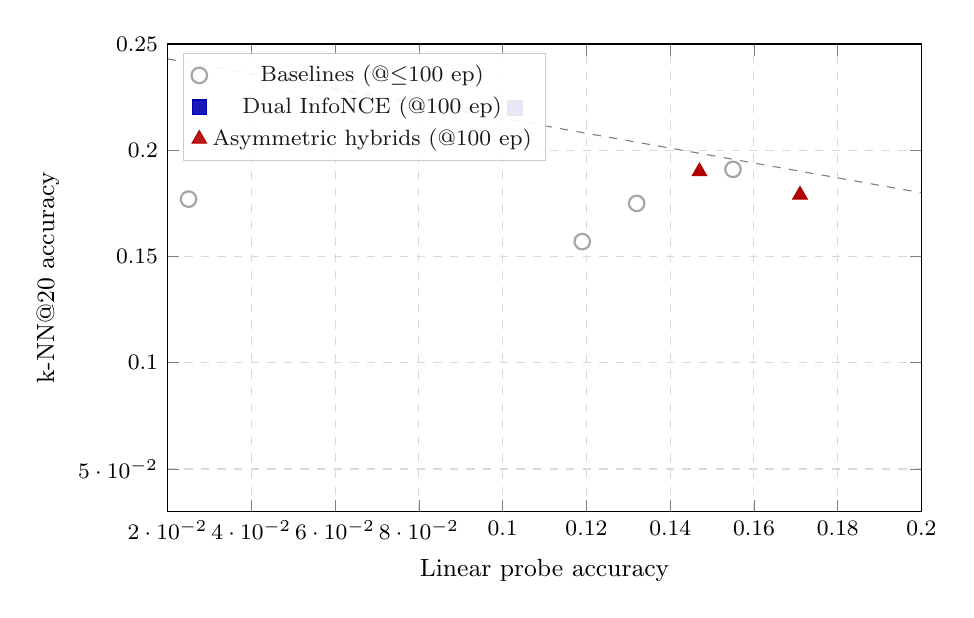
\begin{tikzpicture}
  \begin{axis}[
    width=0.92\linewidth,
    height=0.62\linewidth,
    xlabel={Linear probe accuracy},
    ylabel={k-NN@20 accuracy},
    xmin=0.02, xmax=0.20,
    ymin=0.03, ymax=0.25,
    grid=major,
    grid style={dashed,gray!30},
    legend style={
      at={(0.02,0.98)},
      anchor=north west,
      font=\footnotesize,
      fill=white,
      fill opacity=0.9,
      draw=gray!40,
    },
    tick label style={font=\footnotesize},
    label style={font=\small},
  ]
    % --- Published-style baselines (@100 ep, preliminary) ---
    \addplot[
      only marks,
      mark=*,
      mark size=2.8pt,
      color=gray!70,
      fill=white,
      thick,
    ] coordinates {
      (0.132, 0.175)  % EMA JEPA @100
      (0.155, 0.191)  % EMA JEPA peak @50
      (0.025, 0.177)  % Uniformity @90
      (0.119, 0.157)  % VICReg curriculum @10
    };
    \addlegendentry{Baselines (@${\leq}$100 ep)}

    % --- InfoNCE family (@100 ep) ---
    \addplot[
      only marks,
      mark=square*,
      mark size=2.6pt,
      color=blue!70!black,
    ] coordinates {
      (0.103, 0.220)  % Dual InfoNCE (~@90)
    };
    \addlegendentry{Dual InfoNCE (@100 ep)}

    % --- Proposed hybrids (@100 ep) ---
    \addplot[
      only marks,
      mark=triangle*,
      mark size=3pt,
      color=red!70!black,
    ] coordinates {
      (0.147, 0.190)  % MVC @30
      (0.171, 0.179)  % SIGReg hybrid @90-100
    };
    \addlegendentry{Asymmetric hybrids (@100 ep)}

    % --- @200 ep: update coordinates when sweep completes ---
    % \addplot[only marks, mark=star, ...] coordinates { (linear, knn) ... };

    % Visual guide: higher linear + higher k-NN is upper-right
    \addplot[gray, dashed, domain=0.02:0.20] {0.25 - 0.35*x};
  \end{axis}
\end{tikzpicture}

  \caption{k-NN vs.\ linear probe trade-off on CIFAR-100 (SmallResNet).
  Hollow gray markers: preliminary baselines at ${\leq}100$ epochs;
  blue square: dual InfoNCE; red triangles: proposed hybrids;
  orange star: placeholder for unified @200-epoch sweep.
  Update coordinates from \texttt{history.json} checkpoints.}
  \label{fig:tradeoff}
\end{figure}

\paragraph{Learning curves (same network).}
Figure~\ref{fig:curves} shows epoch-wise k-NN and linear accuracy for
representative methods trained on the same architecture.
We include dual InfoNCE, InfoNCE+SIGReg, and EMA-JEPA as reference curves;
dashed vertical line marks epoch~100 when continuing to 200.

\begin{figure}[t]
  \centering
  \fbox{\parbox{0.92\linewidth}{\centering\vspace{2.2cm}
    \small\textbf{[Figure placeholder]}\\
    Two-panel plot: (left) k-NN@20 vs.\ epoch,
    (right) linear accuracy vs.\ epoch.\\
    Generate with \texttt{scripts/plot\_ablation\_curves.py}
    from checkpoint histories.\vspace{2.2cm}}}
  \caption{Training curves at 10-epoch intervals (SmallResNet, CIFAR-100).
  To be populated from the 200-epoch ablation sweep.}
  \label{fig:curves}
\end{figure}
